\section{Auswertung}
\label{sec:Auswertung}

\subsection{Verstärkungsgeraden}
\label{sec:a1}
Im Folgenden sollen mithilfe der gemessenen Frequenzen und Verstärkungsgrade 
die Leerlaufverstärkung, die Grenzfrequenz und das Bandbreitenprodukt ermittelt 
werden. Es wird die Frequenz gegen die Verstärkung in einem doppelt-logarithmischen 
Diagramm aufgetragen, dabei wird zwischen einem Plateaubereich und einem
abfallenden Bereich unterschieden. Die Leerlaufverstärkung ist jene, bei der der
Operationsvertärker ideal arbeiten kann. Für einen limitierten Frequenzbereich 
ist diese konstant und lässt sich daher durch Mittelung errechnen (Plateaubereich).
Ab der Grenzfrequenz ist der Operationsverstärker außerhalb des idealen 
Arbeitsbereiches und im Diagramm stellt sich ein Abfall ein. Für eine lineare
Regression wird aufgrund der logarithmischen Darstellung ein fit der Form 
\begin{equation*}
    V = n \cdot f^m
\end{equation*}
erstellt. Hierbei ist V die frequenzabhängige Verstärkung. Für die Ermittlung 
der Grenzfrequenzen wird der Punkt berechnet, wo $V =V_0 / \sqrt(2)$, bzw. der 
Schnittpunkt beider Geraden erreicht ist ($V_0$ sei die Leerlaufverstärkung).
In den Plots \autoref{fig:pl1}, \autoref{fig:pl2}, \autoref{fig:pl3} und \autoref{fig:pl4} sind die Daten zu 
sehen.
\begin{figure}[H]
    \centering
        \centering
        \includegraphics[width=0.75\textwidth]{build/L1.pdf}
        \caption{Frequenzgang aus der ersten Messung bei $R_1 = \qty{10}{\kilo\ohm}$
        und $R_2 = \qty{15}{\kilo\ohm}$ des invertierenden-gegengekoppelten-
        Linearverstärkers.}
    \hfill
    \label{fig:pl1}
\end{figure}
\begin{figure}[H]
    \centering
        \centering
        \includegraphics[width=0.75\textwidth]{build/L2.pdf}
        \caption{Frequenzgang aus der zweiten Messung bei $R_1 = \qty{1}{\kilo\ohm}$
        und $R_2 = \qty{10}{\kilo\ohm}$ des invertierenden-gegengekoppelten-
        Linearverstärkers.}
    \hfill
    \label{fig:pl2}
\end{figure}
\begin{figure}[H]
    \centering
        \centering
        \includegraphics[width=0.75\textwidth]{build/L3.pdf}
        \caption{Frequenzgang aus der dritten Messung bei $R_1 = \qty{10}{\kilo\ohm}$
        und $R_2 = \qty{47}{\kilo\ohm}$ des invertierenden-gegengekoppelten-
        Linearverstärkers.}
    \hfill
    \label{fig:pl3}
\end{figure}
\begin{figure}[H]
    \centering
        \centering
        \includegraphics[width=0.75\textwidth]{build/L4.pdf}
        \caption{Frequenzgang aus der vierten Messung bei $R_1 = \qty{15}{\kilo\ohm}$
        und $R_2 = \qty{47}{\kilo\ohm}$ des invertierenden-gegengekoppelten-
        Linearverstärkers.}
    \hfill
    \label{fig:pl4}
\end{figure}
\noindent Es ergeben sich die Werte aus \autoref{tab:5}. Für einen Vergleich 
der bestimmten Werte durch das Experiment wird zusätzlich die theoretische 
Verstärkung durch den Quotienten der Widerstände berechnet.
\begin{table}[H]
    \centering
    \caption{Experimentell ermittelte Ergebnisse.}
    \label{tab:5}
    \sisetup{table-format=1.2}
    \begin{tblr}{
        colspec = {S[table-format=1.0] S[table-format=1.4] S[table-format=2.4] S[table-format=3.2] S[table-format=3.2]},
        row{1} = {guard, mode=math},
        column{2} = {halign=c},  % Zentriere Spalte 2
        column{3} = {halign=c},  % Zentriere Spalte 3
        column{4} = {halign=c},  % Zentriere Spalte 4
        column{5} = {halign=c},  % Zentriere Spalte 5
    }
    \toprule
    \text{Messung} & V_{exp} & V_{theo} & f \mathbin{/} \unit{\kilo\hertz} & B \mathbin{/} \unit{\kilo\hertz}\\
    \midrule
    1 & 1.4857 & 1.5   & 116.11 & 172.50 \\
    2 & 9.7143 & 10.0  & 10.45 & 101.49 \\
    3 & 4.9841 & 4.7   & 44.15 & 220.04 \\
    4 & 3.4286 & 3.133 & 77.63 & 266.15 \\  
    \bottomrule
    \end{tblr}
\end{table}
\noindent Die Daten aus den vier Messungen sind \autoref{tab:1}, \autoref{tab:2},
\autoref{tab:3} und \autoref{tab:4} zu entnehmen.
\vspace{0.5cm}
\\
\begin{minipage}{0.5\linewidth}
    \centering
    \captionof{table}{Erste Messung.}
    \label{tab:1}
    \sisetup{table-format=1.2}
    \begin{tblr}{
        colspec = {S[table-format=3.0] S S[table-format=3.2]},
        row{1} = {guard, mode=math},
    }
    \toprule
    f \mathbin{/} \unit{\kilo\hertz} & U_{out} \mathbin{/} \unit{\volt} & \varphi \mathbin{/} \si{\degree}\\
    \midrule
    0.3 & 1.56 & 180 \\
    0.7 & 1.56 & 180 \\
    1   & 1.56 & 180 \\
    3   & 1.56 & 180 \\
    7   & 1.56 & 180 \\
    10  & 1.56 & 180 \\
    30  & 1.56 & 180 \\
    70  & 1.56 & -120 \\
    100 & 1.30 & -100 \\
    300 & 0.53 &     \\
    700 & 0.28 &     \\
    \bottomrule
    \end{tblr}
\end{minipage}
\hfill
\begin{minipage}{0.5\linewidth}
    \centering
    \captionof{table}{Zweite Messung.}
    \label{tab:2}
    \sisetup{table-format=1.2}
    \begin{tblr}{
        colspec = {S[table-format=3.0] S S[table-format=3.2]},
        row{1} = {guard, mode=math},
    }
    \toprule
    f \mathbin{/} \unit{\kilo\hertz} & U_{out} \mathbin{/} \unit{\volt} & \varphi \mathbin{/} \si{\degree}\\
    \midrule
    0.3 & 10.2 & 180 \\
    0.7 & 10.2 & 180 \\
    1   & 10.2 & 180 \\
    3   & 10.2 & 175 \\
    7   & 10.2 & 170 \\
    10  & 10.2 & 160 \\
    30  & 1.56 & -90 \\
    70  & 1.56 & \\
    100 & 1.30 & \\
    \bottomrule
    \end{tblr}
\end{minipage}

\vspace{0.5cm}

\noindent
\begin{minipage}{0.5\linewidth}
    \centering
    \captionof{table}{Dritte Messung.}
    \label{tab:3}
    \sisetup{table-format=1.2}
    \begin{tblr}{
        colspec = {S[table-format=3.0] S S[table-format=3.2]},
        row{1} = {guard, mode=math},
    }
    \toprule
    f \mathbin{/} \unit{\kilo\hertz} & U_{out} \mathbin{/} \unit{\volt} & \varphi \mathbin{/} \si{\degree}\\
    \midrule
    0.3 & 5.3 & -180 \\
    0.7 & 5.3 & -180 \\
    1   & 5.2 & -180 \\
    3   & 5.2 & -178 \\
    7   & 5.2 & -177 \\
    10  & 5.2 & -175 \\
    30  & 4.8 & -130 \\
    70  & 2.8 & -100 \\
    100 & 2.0 & -90 \\
    \bottomrule
    \end{tblr}
\end{minipage}
\hfill
\begin{minipage}{0.5\linewidth}
    \centering
    \captionof{table}{Vierte Messung.}
    \label{tab:4}
    \sisetup{table-format=1.2}
    \begin{tblr}{
        colspec = {S[table-format=3.0] S S[table-format=3.2]},
        row{1} = {guard, mode=math},
    }
    \toprule
    f \mathbin{/} \unit{\kilo\hertz} & U_{out} \mathbin{/} \unit{\volt} & \varphi \mathbin{/} \si{\degree}\\
    \midrule
    0.3 & 3.6 & -178 \\
    0.7 & 3.6 & -178 \\
    1   & 3.6 & -178 \\
    3   & 3.6 & -178 \\
    7   & 3.6 & -176 \\
    10  & 3.6 & -180 \\
    30  & 3.8 & -170 \\
    70  & 2.8 & -120 \\
    100 & 2.2 &  \\
    \bottomrule
    \end{tblr}
\end{minipage}



\subsection{Ermittlung der Grundschaltung durch die Phase}
\label{sec:a2}
Es wird die Phasenbeziehung in Abhängigkeit der Frequenz aufgetragen, die 
Ergebnisse sind den \autoref{fig:pl5} bis \autoref{fig:pl8} zu sehen. 
Im Wesentlichen verändert sich die Phase um $\qty{90}{\degree}$, ausgehend 
von der invertierenden Grundschaltung von $\qty{180}{\degree}$ oder 
$\qty{-180}{\degree}$. Die charakteristischen Verläufe zeigen das klassische
Verhalten eines Tiefpasses.
\begin{figure}[H]
    \centering
        \centering
        \includegraphics[width=0.68\textwidth]{build/LP1.pdf}
        \caption{Verlauf der Phase aus der ersten Messung bei $R_1 = \qty{10}{\kilo\ohm}$
        und $R_2 = \qty{15}{\kilo\ohm}$ des invertierenden-gegengekoppelten-
        Linearverstärkers.}
    \hfill
    \label{fig:pl5}
\end{figure}
\begin{figure}[H]
    \centering
        \centering
        \includegraphics[width=0.68\textwidth]{build/LP2.pdf}
        \caption{Verlauf der Phase aus der zweiten Messung bei $R_1 = \qty{1}{\kilo\ohm}$
        und $R_2 = \qty{10}{\kilo\ohm}$ des invertierenden-gegengekoppelten-
        Linearverstärkers.}
    \hfill
    \label{fig:pl6}
\end{figure}
\begin{figure}[H]
    \centering
        \centering
        \includegraphics[width=0.68\textwidth]{build/LP3.pdf}
        \caption{Verlauf der Phase aus der dritten Messung bei $R_1 = \qty{10}{\kilo\ohm}$
        und $R_2 = \qty{47}{\kilo\ohm}$ des invertierenden-gegengekoppelten-
        Linearverstärkers.}
    \hfill
    \label{fig:pl7}
\end{figure}
\begin{figure}[H]
    \centering
        \centering
        \includegraphics[width=0.68\textwidth]{build/LP4.pdf}
        \caption{Verlauf der Phase aus der vierten Messung bei $R_1 = \qty{15}{\kilo\ohm}$
        und $R_2 = \qty{47}{\kilo\ohm}$ des invertierenden-gegengekoppelten-
        Linearverstärkers.}
    \hfill
    \label{fig:pl8}
\end{figure}



\subsection{Proportionalitätsprüfung am Umkehr-Integrator}
\label{sec:a3}
Für den Umkehrintegrator werden zu Frequenzen am Eingang die Ausgangssignale 
gemessen. Der Theorie zufolge sollte sich für die Verstärkung eine Proportionalität 
der Steigung von $1/f$ gelten. Werden die Frequenzen gegen die zugehörige 
Verstärkung nun in einem (doppel)logarithmischen Diagramm aufgetragen, sollte 
sich eine Steigung von $m = -1$ ergeben. Die Messwerte zur Umkehr-Integrator-
Schaltung befinden sich in \autoref{tab:4}. Die Ausgleichsgerade ist in 
\autoref{fig:pl9} zu sehen. Die Steigung beträgt
\begin{align*}
    m &= -0.9193 \pm 0.0206.
\end{align*}
\begin{figure}[H]
    \centering
        \centering
        \includegraphics[width=0.75\textwidth]{build/UI.pdf}
        \caption{Lineare Regression zur Ermittlung des Verhältnisses zwischen 
        Ein-und Ausgangsspannung.}
    \hfill
    \label{fig:pl9}
\end{figure}
\noindent Für die Schaltung wurden ein Widerstand $R_1 = \qty{10}{\kilo\ohm}$ und 
ein Kondensator $C = \qty{10}{\nano\farad}$ genutzt. Darüber hinaus wurde parallel 
zum Kondensator noch ein weiterer Widerstand $R_2 = \qty{10}{\kilo\ohm}$ genutzt,
dieser verhindert, dass die Gleichspannungsverstärkung den Integrator in die 
Sättigung treibt.
\begin{table}[H]
    \centering
    \captionof{table}{Messwerte für den Umkehr-Integrator.}
    \label{tab:4}
    \sisetup{table-format=1.2}
    \begin{tblr}{
        colspec = {S[table-format=3.0] S[table-format=3.2]},
        row{1} = {guard, mode=math},
    }
    \toprule
    f \mathbin{/} \unit{\kilo\hertz} & U_{out} \mathbin{/} \unit{\volt} \\
    \midrule
    0.1 & 12.5 \\
    0.2 & 7.6  \\
    0.4 & 4.4  \\
    0.8 & 2.6  \\
    1.0 & 1.7  \\
    2.0 & 0.9  \\
    4.0 & 0.45  \\
    8.0 & 0.24  \\
    10.0 & 0.19  \\
    20.0 & 0.12  \\
    \bottomrule
    \end{tblr}
\end{table}
\noindent Weiter sollten die Ausgangssignale für die digital abgespeichert werden.
Die Bildschirmfotos sind in \autoref{fig:ss1}, \autoref{fig:ss2} und \autoref{fig:ss3}
zu sehen. Die gelben Verläufe auf dem Oszilloskop sind die angelegten Sinus-,
Dreieck- und Rechteckspannungen. In grün sind die Funktionen zu sehen, welche 
durch den Integrator erzeugt werden. 
\begin{figure}[H]
    \centering
        \centering
        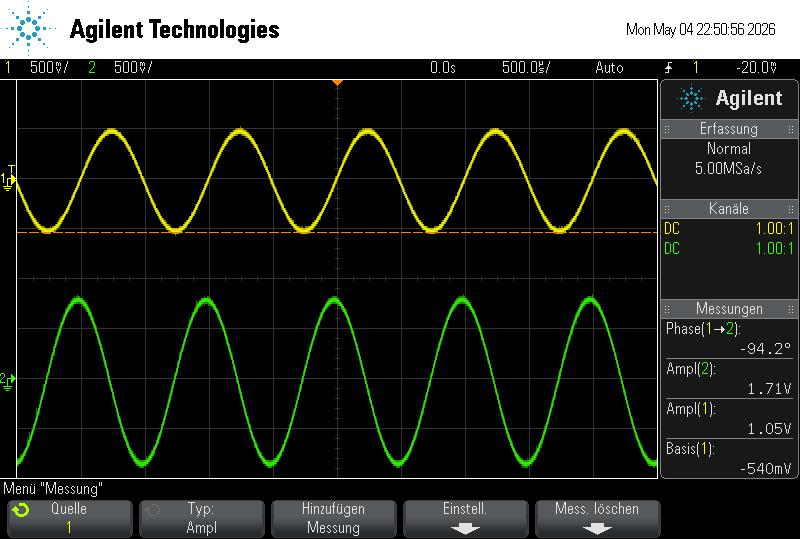
\includegraphics[width=0.8\textwidth]{Bilder/scope_0.png}
        \caption{Bildschirmaufnahme des Sinussignals.}
    \hfill
    \label{fig:ss1}
\end{figure}
\begin{figure}[H]
    \centering
        \centering
        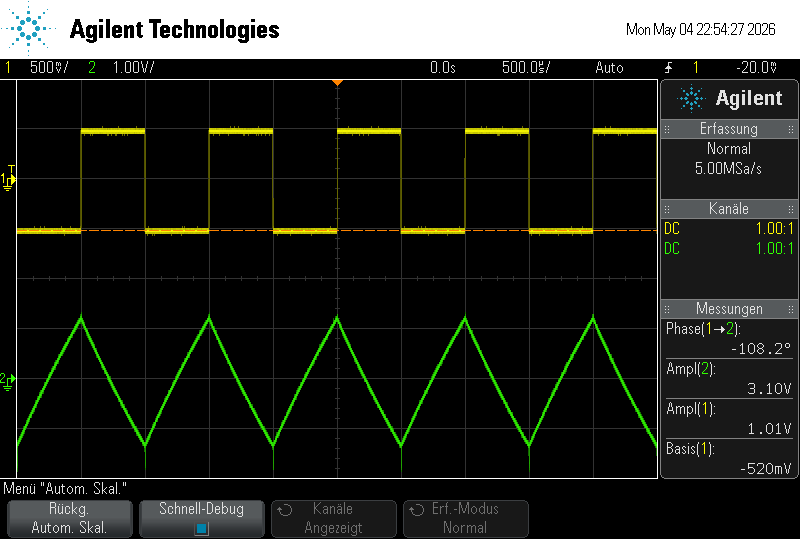
\includegraphics[width=0.8\textwidth]{Bilder/scope_2.png}
        \caption{Bildschirmaufnahme des Rechtecksignals.}
    \hfill
    \label{fig:ss2}
\end{figure}
\begin{figure}[H]
    \centering
        \centering
        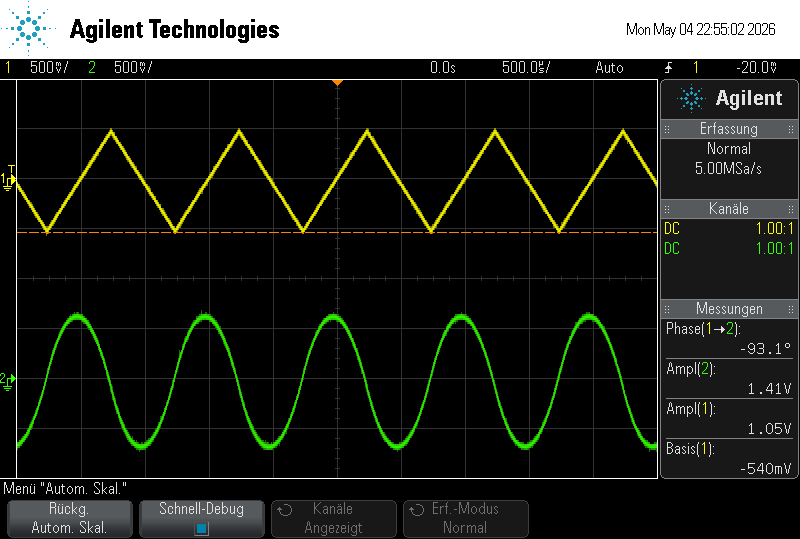
\includegraphics[width=0.8\textwidth]{Bilder/scope_4.png}
        \caption{Bildschirmaufnahme des Dreiecksignals.}
    \hfill
    \label{fig:ss3}
\end{figure}



\subsection{Proportionalitätsprüfung am Umkehr-Differenzierer}
\label{sec:a4}
Analog zu \autoref{sec:a3} soll für den Umkehr-Differenzierer verfahren werden.
Für diesen gilt im Gegensatz zum Integrator eine Proportionalität von $f$ 
zu der Verstärkung. Das entspricht einer Steigung von $m=1$, wenn die Verstärkung 
$V$ gegen die Frequenz $f$ in einem (doppel)logarithmischen Diagramm aufgetragen 
wird. Die Messwerte für diesen Teil befinden sich in \autoref{tab:5} und die 
Ausgleichsgerade in \autoref{fig:pl10}. Für die Steigung ergibt sich ein Wert 
von 
\begin{align*}
    m = 0.8414 \pm 0.0428.
\end{align*}
\begin{figure}[H]
    \centering
        \centering
        \includegraphics[width=0.75\textwidth]{build/UD.pdf}
        \caption{Lineare Regression zur Ermittlung des Verhältnisses zwischen 
        Ein-und Ausgangsspannung.}
    \hfill
    \label{fig:pl10}
\end{figure}
\begin{table}[H]
    \centering
    \captionof{table}{Messwerte für den Umkehr-Differenzierer.}
    \label{tab:5}
    \sisetup{table-format=1.2}
    \begin{tblr}{
        colspec = {S[table-format=3.0] S[table-format=3.2]},
        row{1} = {guard, mode=math},
    }
    \toprule
    f \mathbin{/} \unit{\kilo\hertz} & U_{out} \mathbin{/} \unit{\milli\volt} \\
    \midrule
    0.1 & 120 \\
    0.2 & 170 \\
    0.4 & 290 \\
    0.8 & 520 \\
    1.0 & 640 \\
    1.2 & 760 \\
    1.4 & 870 \\
    1.6 & 1000 \\
    1.8 & 1310 \\
    2.0 & 1170 \\
    2.2 & 1770 \\
    \bottomrule
    \end{tblr}
\end{table}
Die Ausgangssignale für die drei unterschiedlichen Spannungen (Sinus, Rechteck 
und Dreieck) befinden sich in \autoref{fig:ss4}, \autoref{fig:ss5} und 
\autoref{fig:ss6}.
\begin{figure}[H]
    \centering
        \centering
        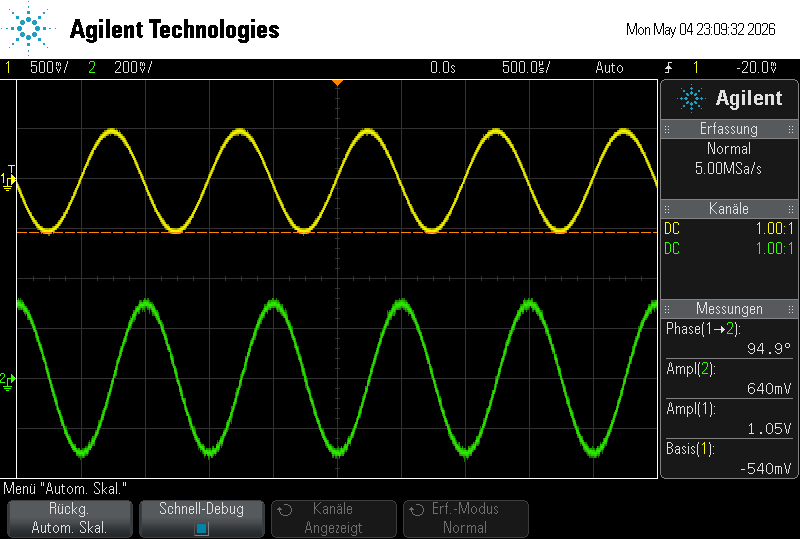
\includegraphics[width=0.8\textwidth]{Bilder/scope_6.png}
        \caption{Bildschirmaufnahme des Sinussignals.}
    \hfill
    \label{fig:ss4}
\end{figure}
\begin{figure}[H]
    \centering
        \centering
        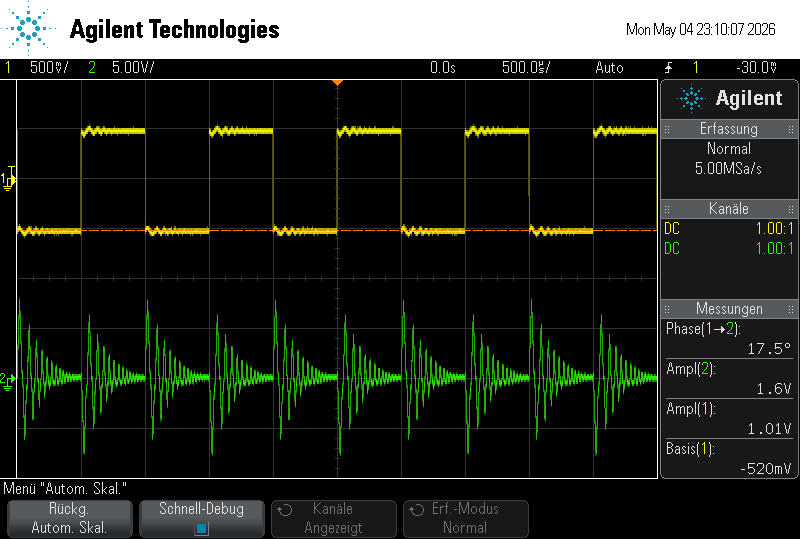
\includegraphics[width=0.8\textwidth]{Bilder/scope_8.png}
        \caption{Bildschirmaufnahme des Rechtecksignals.}
    \hfill
    \label{fig:ss5}
\end{figure}
\begin{figure}[H]
    \centering
        \centering
        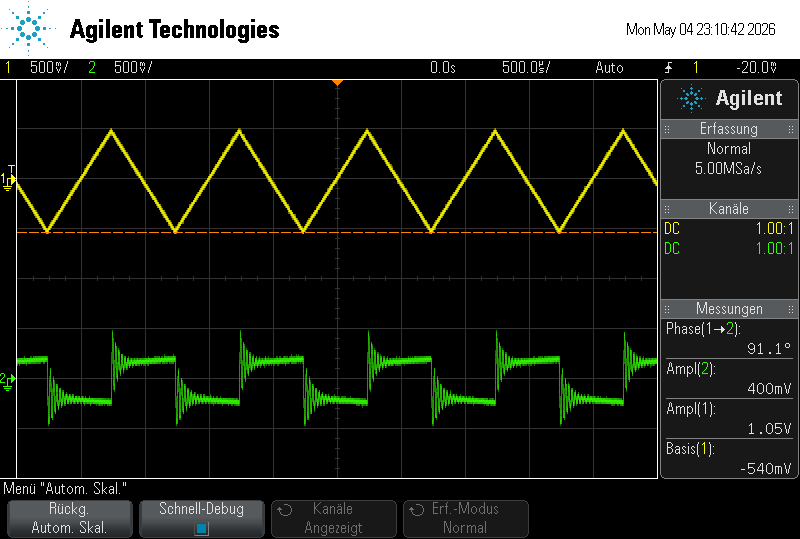
\includegraphics[width=0.8\textwidth]{Bilder/scope_10.png}
        \caption{Bildschirmaufnahme des Dreiecksignals.}
    \hfill
    \label{fig:ss6}
\end{figure}



\subsection{Nicht-invertierende-Schmitt-Trigger und Kippspannungen}
Für den nicht-invertierenden-Schmitt-Trigger werden $R_1 = \qty{10}{\kilo\ohm}$
und $R_2 = \qty{100}{\kilo\ohm}$ bei einer Ausgangsspannung von $U_S = \pm
\qty{15}{\volt}$ genutzt. Weiter wird von dem Generator ein Sinussignal bei
einer Frequenz von $\qty{100}{\hertz}$ ausgegeben. 
Die obere bzw. untere Kippspannung berechnet sich zu
\begin{equation*}
    U_{\text{kipp}} = U_S \cdot \frac{R_1}{R_1 + R_2} = \qty{\pm 1,364}{\volt}.
\end{equation*}
Die gesamte Hysteresebreite (Differenz zwischen oberer und unterer Kippspannung)
beträgt damit
\begin{equation*}
    \Delta U_{\text{theo}} = 2 \cdot U_{\text{kipp}} = \qty{2,727}{\volt}.
\end{equation*}
Durch empirische Bestimmung ergibt sich experimentell ein Wert von 
\begin{equation*}
    \Delta U_{\text{exp}} = \qty{2.736 \pm 0.002}{\volt}.
\end{equation*}